\chapter{Desenvolvimento}
\label{cap:desenvolvimento}
Neste capítulo, é apresentado as etapas de desenvolvimento do projeto.

\section{Levantamento das Estórias}

As estórias foram identificadas, analisadas e descritas abaixo:

\begin{itemize}
	\item \textbf{Estória 01: Cadastrar Catador}\par
Descrição: Permite a criação do usuário responsável pelo recolhimento do material descartado.

	\item \textbf{Estória 02: Cadastrar Separador}\par
Descrição: Permite a criação do usuário responsável pelo descarte do material.

	\item \textbf{Estória 03: Efetuar login}\par
Descrição: Autoriza o acesso às funcionalidades do sistema. 

	\item \textbf{Estória 04: Recuperar senha }\par
Descrição: Possibilita que o usuário redefina a senha.

	\item \textbf{Estória 05: Tirar dúvidas }\par
Descrição: Esclarece sobre a definição dos perfis. 

	\item \textbf{Estória 06: Solicitar recolhimento}\par
Descrição: Requisita a coleta do material descartado.

	\item \textbf{Estória 07: Realizar logoff}\par
Descrição: Permite que o usuário saia do sistema.

	\item \textbf{Estória 08: Lembrar login}\par
Descrição: Permite que os dados de autenticação do usuário, fiquem salvos na tela de \textit{login}.

	\item \textbf{Estória 9: Traçar rota da coleta}\par
Descrição: Possibilita que o usuário visualize no mapa a duração e a distância do trajeto a ser percorrido.

	\item \textbf{Estória 10: Visualizar mapa}\par
Descrição: Facilitar a visualização da localização.

	\item \textbf{Estória 11: Escolher tipo de material}\par
Descrição: Informar qual tipo de material reciclável será descartado.

	\item \textbf{Estória 12: Informar localização}\par
Descrição: Informar a localização para o descarte do material.
\end{itemize}


\section{Diagramas do Modelo Proposto}

\subsection{Diagrama de Classes}

Na construção do diagrama de classes foi analisada as principais classes do sistema, suas características, seus relacionamentos e suas funcionalidades. É possível observar através da \autoref{fig:classe}, a estrutura do desenvolvimento do sistema.

%%%%%%%%%%%%%%%%%%%% Figure/Image No: 8 starts here %%%%%%%%%%%%%%%%%%%%

\begin{figure}[H]
	\begin{Center}
		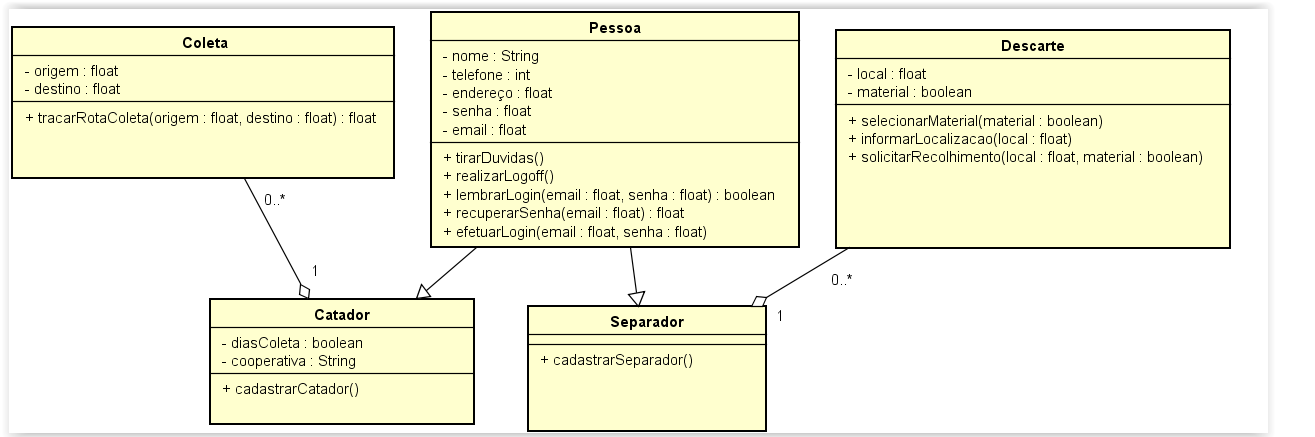
\includegraphics[width=6.4in,height=2.77in]{./media/image35.png}
	\end{Center}
	\caption{Diagrama de Classes}
	\label{fig:classe}
\end{figure}

%%%%%%%%%%%%%%%%%%%% Figure/Image No: 8 Ends here %%%%%%%%%%%%%%%%%%%%

Na \autoref{fig:classe} citada acima podemos observar o Diagrama de Classes utilizado para a construção do aplicativo.

As classes Catador e Separador são extensões da classe Pessoa, que tem como objetivo informar seus dados, tirar dúvidas sobre a definição dos perfis, criar uma conta perfil, redefinir a senha esquecida, efetuar \textit{login}, salvar os dados do \textit{login} e realizar \textit{logoff}.

A classe Catador que faz parte de uma das contas perfil, é responsável pelo cadastro do usuário catador. Este usuário é encarregado por traçar a rota da coleta e recolher o material descartado.

A classe Separador que faz parte de uma das contas perfil, é responsável pelo cadastro do usuário separador. Ao informar sua localização e o tipo de material, o usuário poderá solicitar o recolhimento do material descartado.

\subsection{Diagrama de Casos de Uso}

Esse parágrafo descreve as funcionalidades do sistema e as interações entre os atores, através da \autoref{fig:casos}. 

%%%%%%%%%%%%%%%%%%%% Figure/Image No: 9 starts here %%%%%%%%%%%%%%%%%%%%

\begin{figure}[H]
	\begin{Center}
		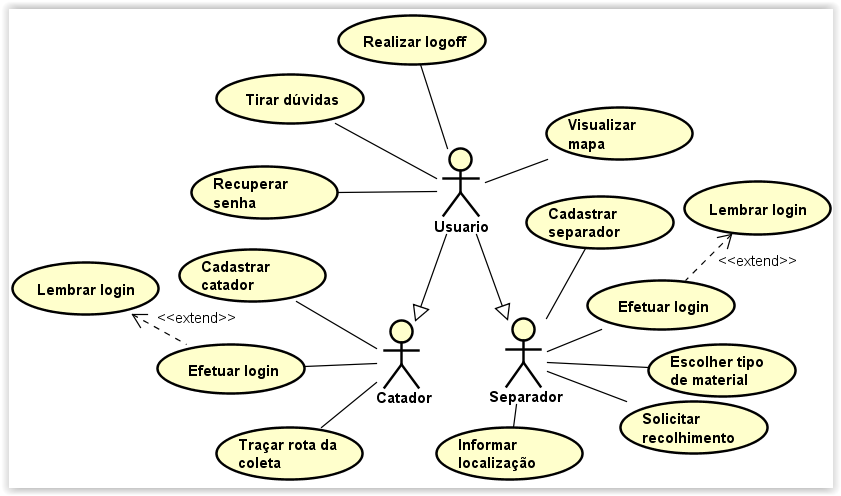
\includegraphics[width=5.12in,height=3.02in]{./media/image32.png}
	\end{Center}
	\caption{Diagrama de Casos de Uso}
	\label{fig:casos}
\end{figure}

%%%%%%%%%%%%%%%%%%%% Figure/Image No: 9 Ends here %%%%%%%%%%%%%%%%%%%%

Na \autoref{fig:casos} citada acima, podemos ver o Diagrama de Casos de Uso. Na tela inicial do aplicativo, o usuário poderá realizar as seguintes funções: logar no APP, cadastrar usuário, tirar dúvidas, efetuar \textit{logoff} e recuperar a senha. Se o usuário ainda não estiver cadastrado, irá se cadastrar no perfil desejado: Catador ou Separador. Caso já tenha cadastro, basta efetuar o \textit{login}, o qual pode ser salvo pelo sistema. Em caso de senha esquecida, o sistema permite a recuperação através do \textit{e-mail}.

A partir da inserção da localização e do tipo de material, o Separador poderá solicitar o recolhimento do rejeito. O Catador recebendo a solicitação do Separador, irá traçar a rota para a coleta do material. 

\paragraph*{5.2.2.1 Especificação dos Casos de Uso}

Esse capítulo é responsável pelo detalhamento das funcionalidades do sistema. O (\autoref{quad:catador}), descreve o passo a passo para o cadastro do usuário Catador.

%%%%%%%%%%%%%%%%%%%% Table No: 4 starts here %%%%%%%%%%%%%%%%%%%%

\begin{quadro}[H]
\caption{Cadastrar Catador}
\label{quad:catador}
\centering
\begin{tabular}{p{1.25in}p{4.50in}}
\hline
%row no:1
\multicolumn{1}{|p{1.25in}}{\textbf{Caso de Uso}} & 
\multicolumn{1}{|p{4.50in}|}{Cadastrar Catador} \\
\hhline{--}
%row no:2
\multicolumn{1}{|p{1.25in}}{\textbf{Descrição}} & 
\multicolumn{1}{|p{4.50in}|}{Permite a criação de perfil usuário denominado catador.} \\
\hhline{--}
%row no:3
\multicolumn{1}{|p{1.25in}}{\textbf{Ator}} & 
\multicolumn{1}{|p{4.50in}|}{Catador} \\
\hhline{--}
%row no:4
\multicolumn{1}{|p{1.25in}}{\textbf{Pré-condições}} & 
\multicolumn{1}{|p{4.50in}|}{Preencher todos os dados solicitados} \\
\hhline{--}
%row no:5
\multicolumn{1}{|p{1.25in}}{\textbf{Pós-condições}} & 
\multicolumn{1}{|p{4.50in}|}{Cadastro do perfil catador no sistema} \\
\hhline{--}
%row no:6
\multicolumn{1}{|p{1.25in}}{\textbf{Fluxo Principal}} & 
\multicolumn{1}{|p{4.50in}|}{\begin{enumerate}[label*={\fontsize{12pt}{12pt}\selectfont \arabic*.}]
	\item Na tela inicial, o usuário solicita o cadastro; \par 	\item Em seguida preenche todos os dados; \par 	\item O sistema valida os dados preenchidos; \par 	\item O cadastro é realizado.
\end{enumerate}} \\
\hhline{--}
%row no:7
\multicolumn{1}{|p{1.25in}}{\textbf{Fluxo de Exceção}} & 
\multicolumn{1}{|p{4.50in}|}{\textbf{Dados incorretos} \par \begin{enumerate}[label*={\fontsize{12pt}{12pt}\selectfont \arabic*.}]
	\item No passo 3 do Fluxo Principal, o usuário não preencheu os dados corretamente, o sistema sinaliza qual campo não foi preenchido.
\end{enumerate} \par \textbf{Dados não cadastrados} \par \begin{enumerate}[label*={\fontsize{12pt}{12pt}\selectfont \arabic*.}]
	\item No passo 3 do Fluxo Principal, o usuário preenche algum campo já cadastrado, o sistema exibe qual campo já foi cadastrado.
\end{enumerate}} \\
\hhline{--}

\end{tabular}
\end{quadro}


%%%%%%%%%%%%%%%%%%%% Table No: 4 ends here %%%%%%%%%%%%%%%%%%%%

O caso de uso Cadastrar Catador (\autoref{quad:catador}), citado acima é responsável por avaliar as ações necessárias para realizar o cadastro do perfil catador. 

O \autoref{qua:separador} descreve o passo a passo para o cadastro do usuário Separador.

%%%%%%%%%%%%%%%%%%%% Table No: 5 starts here %%%%%%%%%%%%%%%%%%%%


\begin{quadro}[H]
\caption{Cadastro Separador}
 \label{qua:separador}			\begin{tabular}{p{1.33in}p{3.96in}}
\hline
%row no:1
\multicolumn{1}{|p{1.33in}}{\textbf{Caso de Uso}} & 
\multicolumn{1}{|p{3.96in}|}{Cadastrar Separador} \\
\hhline{--}
%row no:2
\multicolumn{1}{|p{1.33in}}{\textbf{Descrição}} & 
\multicolumn{1}{|p{3.96in}|}{Permite a criação de perfil usuário denominado separador.} \\
\hhline{--}
%row no:3
\multicolumn{1}{|p{1.33in}}{\textbf{Ator}} & 
\multicolumn{1}{|p{3.96in}|}{Separador} \\
\hhline{--}
%row no:4
\multicolumn{1}{|p{1.33in}}{\textbf{Pré-condições}} & 
\multicolumn{1}{|p{3.96in}|}{Preencher todos os dados solicitados } \\
\hhline{--}
%row no:5
\multicolumn{1}{|p{1.33in}}{\textbf{Pós-condições}} & 
\multicolumn{1}{|p{3.96in}|}{Cadastro do perfil separador no sistema} \\
\hhline{--}
%row no:6
\multicolumn{1}{|p{1.33in}}{\textbf{Fluxo Principal}} & 
\multicolumn{1}{|p{3.96in}|}{\begin{enumerate}[label*={\fontsize{12pt}{12pt}\selectfont \arabic*.}]
	\item Na tela inicial, o usuário solicita o cadastro; \par 	\item Em seguida, preenche todos os dados; \par 	\item O sistema verifica os dados; \par 	\item O cadastro é realizado.
\end{enumerate}} \\
\hhline{--}

\end{tabular}
 \end{quadro}

%%%%%%%%%%%%%%%%%%%% Table No: 5 ends here %%%%%%%%%%%%%%%%%%%%

O caso de uso Cadastrar Separador (\autoref{qua:separador}), citado acima é responsável por avaliar as ações necessárias para realizar o cadastro do perfil separador. 

O \autoref{quad:login} descreve o passo a passo para efetuar o \textit{login}.

%%%%%%%%%%%%%%%%%%%% Table No: 6 starts here %%%%%%%%%%%%%%%%%%%%


\begin{quadro}[H]
\caption{Efetuar Login}
\label{quad:login}
\centering
\begin{tabular}{p{1.35in}p{3.94in}}
\hline
%row no:1
\multicolumn{1}{|p{1.35in}}{\textbf{Caso de Uso}} & 
\multicolumn{1}{|p{3.94in}|}{Efetuar \textit{login}} \\
\hhline{--}
%row no:2
\multicolumn{1}{|p{1.35in}}{\textbf{Descrição}} & 
\multicolumn{1}{|p{3.94in}|}{Permite acesso às funcionalidades do sistema.} \\
\hhline{--}
%row no:3
\multicolumn{1}{|p{1.35in}}{\textbf{Ator}} & 
\multicolumn{1}{|p{3.94in}|}{Catador e Separador} \\
\hhline{--}
%row no:4
\multicolumn{1}{|p{1.35in}}{\textbf{Pré-condições}} & 
\multicolumn{1}{|p{3.94in}|}{O usuário deve estar cadastrado no sistema.} \\
\hhline{--}
%row no:5
\multicolumn{1}{|p{1.35in}}{\textbf{Pós-condições}} & 
\multicolumn{1}{|p{3.94in}|}{O usuário estará logado no sistema.} \\
\hhline{--}
%row no:6
\multicolumn{1}{|p{1.35in}}{\textbf{Fluxo Principal}} & 
\multicolumn{1}{|p{3.94in}|}{\begin{enumerate}[label*={\fontsize{12pt}{12pt}\selectfont \arabic*.}]
	\item Na tela inicial o usuário, informa o \textit{e-mail} e senha; \par 	\item Em seguida realiza o \textit{login}; \par 	\item O sistema verifica os dados; \par 	\item O usuário acessa a aplicação.
\end{enumerate}} \\
\hhline{--}
%row no:7
\multicolumn{1}{|p{1.35in}}{\textbf{Fluxo de Exceção}} & 
\multicolumn{1}{|p{3.94in}|}{\textbf{Usuário ou senha inválidos} \par \begin{enumerate}[label*={\fontsize{12pt}{12pt}\selectfont \arabic*.}]
	\item No passo 1, o usuário informa \textit{e-mail} e/ou senha não cadastrados; \par 	\item O sistema informa que os dados estão incorretos.
\end{enumerate} \par \textbf{Campo nulo} \par \begin{enumerate}[label*={\fontsize{12pt}{12pt}\selectfont \arabic*.}]
	\item No passo 1, o usuário não preenche algum campo; \par 	\item O sistema informa qual campo não foi preenchido; \par 	\item Retorna para o passo 1.
\end{enumerate}} \\
\hhline{--}

\end{tabular}
\end{quadro}

%%%%%%%%%%%%%%%%%%%% Table No: 6 ends here %%%%%%%%%%%%%%%%%%%%

O caso de uso Efetuar Login (\autoref{quad:login}), citado acima é responsável por avaliar as ações necessárias para realizar o \textit{login }do usuário. 

O \autoref{quad:recusenha} descreve o passo a passo para a recuperação da senha.

%%%%%%%%%%%%%%%%%%%% Table No: 7 starts here %%%%%%%%%%%%%%%%%%%%


\begin{quadro}[H]
\caption{Recuperar Senha}
\label{quad:recusenha}
\centering
\begin{tabular}{p{1.35in}p{3.84in}}
\hline
%row no:1
\multicolumn{1}{|p{1.35in}}{\textbf{Caso de Uso}} & 
\multicolumn{1}{|p{3.84in}|}{Recuperar senha} \\
\hhline{--}
%row no:2
\multicolumn{1}{|p{1.35in}}{\textbf{Descrição}} & 
\multicolumn{1}{|p{3.84in}|}{Redefinir senha} \\
\hhline{--}
%row no:3
\multicolumn{1}{|p{1.35in}}{\textbf{Ator}} & 
\multicolumn{1}{|p{3.84in}|}{Separador e Catador} \\
\hhline{--}
%row no:4
\multicolumn{1}{|p{1.35in}}{\textbf{Pré-condições}} & 
\multicolumn{1}{|p{3.84in}|}{O usuário deve estar cadastrado no sistema.} \\
\hhline{--}
%row no:5
\multicolumn{1}{|p{1.35in}}{\textbf{Pós-condições}} & 
\multicolumn{1}{|p{3.84in}|}{A senha será recuperada após o preenchimento do \textit{e-mail}.} \\
\hhline{--}
%row no:6
\multicolumn{1}{|p{1.35in}}{\textbf{Cenário Principal}} & 
\multicolumn{1}{|p{3.84in}|}{\begin{enumerate}[label*={\fontsize{12pt}{12pt}\selectfont \arabic*.}]
	\item O usuário solicita a recuperação da senha; \par 	\item Em seguida, informa o \textit{e-mail}; \par 	\item Um \textit{e-mail }para a redefinição da senha é enviado para o usuário. 
\end{enumerate}} \\
\hhline{--}

\end{tabular}
\end{quadro}

%%%%%%%%%%%%%%%%%%%% Table No: 7 ends here %%%%%%%%%%%%%%%%%%%%

O caso de uso Recuperar Senha (\autoref{quad:recusenha}), citado acima é responsável por avaliar as ações necessárias para realizar a redefinição da senha esquecida pelo usuário.

O \autoref{quad:duvida} descreve o passo a passo para tirar dúvidas.

%%%%%%%%%%%%%%%%%%%% Table No: 8 starts here %%%%%%%%%%%%%%%%%%%%


\begin{quadro}[H]
\caption{Tirar Dúvidas}
\label{quad:duvida}
\centering
\begin{tabular}{p{1.35in}p{4.33in}}
\hline
%row no:1
\multicolumn{1}{|p{1.35in}}{\textbf{Caso de Uso}} & 
\multicolumn{1}{|p{4.33in}|}{Tirar dúvidas} \\
\hhline{--}
%row no:2
\multicolumn{1}{|p{1.35in}}{\textbf{Descrição}} & 
\multicolumn{1}{|p{4.33in}|}{Explicar a definição dos perfis.} \\
\hhline{--}
%row no:3
\multicolumn{1}{|p{1.35in}}{\textbf{Ator}} & 
\multicolumn{1}{|p{4.33in}|}{Separador e Catador} \\
\hhline{--}
%row no:4
\multicolumn{1}{|p{1.35in}}{\textbf{Pré-condições}} & 
\multicolumn{1}{|p{4.33in}|}{O usuário não precisa ser cadastrado ou estar logado no sistema.} \\
\hhline{--}
%row no:5
\multicolumn{1}{|p{1.35in}}{\textbf{Pós-condições}} & 
\multicolumn{1}{|p{4.33in}|}{O sistema deve ser iniciado.} \\
\hhline{--}
%row no:6
\multicolumn{1}{|p{1.35in}}{\textbf{Cenário Principal}} & 
\multicolumn{1}{|p{4.33in}|}{\begin{enumerate}[label*={\fontsize{12pt}{12pt}\selectfont \arabic*.}]
	\item O usuário clica no ícone de dúvidas; \par 	\item O sistema redireciona o usuário para a tela informativa.
\end{enumerate}} \\
\hhline{--}

\end{tabular}
\end{quadro}

%%%%%%%%%%%%%%%%%%%% Table No: 8 ends here %%%%%%%%%%%%%%%%%%%%

O caso de uso Tirar Dúvidas (\autoref{quad:duvida}), citado acima é responsável por avaliar as ações necessárias para esclarecer a definição dos perfis. 

O \autoref{quad:logoff} descreve o passo a passo para realizar \textit{logoff}.

%%%%%%%%%%%%%%%%%%%% Table No: 9 starts here %%%%%%%%%%%%%%%%%%%%

\begin{quadro}[H]
\caption{Realizar Logoff}
\label{quad:logoff}
\centering
\begin{tabular}{p{1.35in}p{3.15in}}
\hline
%row no:1
\multicolumn{1}{|p{1.35in}}{\textbf{Caso de Uso}} & 
\multicolumn{1}{|p{3.15in}|}{Realizar logoff} \\
\hhline{--}
%row no:2
\multicolumn{1}{|p{1.35in}}{\textbf{Descrição}} & 
\multicolumn{1}{|p{3.15in}|}{Sair do aplicativo} \\
\hhline{--}
%row no:3
\multicolumn{1}{|p{1.35in}}{\textbf{Ator}} & 
\multicolumn{1}{|p{3.15in}|}{Separador e Catador} \\
\hhline{--}
%row no:4
\multicolumn{1}{|p{1.35in}}{\textbf{Pré-condições}} & 
\multicolumn{1}{|p{3.15in}|}{O usuário precisa estar cadastrado no sistema.} \\
\hhline{--}
%row no:5
\multicolumn{1}{|p{1.35in}}{\textbf{Pós-condições}} & 
\multicolumn{1}{|p{3.15in}|}{O usuário é deslogado do sistema.} \\
\hhline{--}
%row no:6
\multicolumn{1}{|p{1.35in}}{\textbf{Cenário Principal}} & 
\multicolumn{1}{|p{3.15in}|}{\begin{enumerate}[label*={\fontsize{12pt}{12pt}\selectfont \arabic*.}]
	\item O usuário solicita a saída da aplicação; \par 	\item O sistema desloga o usuário.
\end{enumerate}} \\
\hhline{--}

\end{tabular}
\end{quadro}

%%%%%%%%%%%%%%%%%%%% Table No: 9 ends here %%%%%%%%%%%%%%%%%%%%

O caso de uso Realizar \textit{Logoff} (\autoref{quad:logoff}), citado acima é responsável por avaliar as ações necessárias para o término do uso do sistema. 

O \autoref{quad:local} descreve o passo a passo para buscar a localização.

%%%%%%%%%%%%%%%%%%%% Table No: 10 starts here %%%%%%%%%%%%%%%%%%%%

\begin{quadro}[H]
\caption{Informar Localização}
\label{quad:local}
\centering
\begin{tabular}{p{1.35in}p{3.94in}}
\hline
%row no:1
\multicolumn{1}{|p{1.35in}}{\textbf{Caso de Uso}} & 
\multicolumn{1}{|p{3.94in}|}{Informar localização} \\
\hhline{--}
%row no:2
\multicolumn{1}{|p{1.35in}}{\textbf{Descrição}} & 
\multicolumn{1}{|p{3.94in}|}{Informar a localização do material descartado.} \\
\hhline{--}
%row no:3
\multicolumn{1}{|p{1.35in}}{\textbf{Ator}} & 
\multicolumn{1}{|p{3.94in}|}{Separador} \\
\hhline{--}
%row no:4
\multicolumn{1}{|p{1.35in}}{\textbf{Pré-condições}} & 
\multicolumn{1}{|p{3.94in}|}{O usuário deve estar cadastrado no sistema.} \\
\hhline{--}
%row no:5
\multicolumn{1}{|p{1.35in}}{\textbf{Pós-condições}} & 
\multicolumn{1}{|p{3.94in}|}{O sistema deve ser executado.} \\
\hhline{--}
%row no:6
\multicolumn{1}{|p{1.35in}}{\textbf{Cenário Principal}} & 
\multicolumn{1}{|p{3.94in}|}{\begin{enumerate}[label*={\fontsize{12pt}{12pt}\selectfont \arabic*.}]
	\item O usuário informa o local para a coleta do material.
\end{enumerate}} \\
\hhline{--}

\end{tabular}
\end{quadro}

%%%%%%%%%%%%%%%%%%%% Table No: 10 ends here %%%%%%%%%%%%%%%%%%%%

O caso de uso Informar Localização (\autoref{quad:local}), citado acima é responsável por avaliar as ações necessárias para a localização do material informada pelo usuário. 

O \autoref{quad:recolhe} descreve o passo a passo para solicitação do recolhimento do material descartado.

%%%%%%%%%%%%%%%%%%%% Table No: 11 starts here %%%%%%%%%%%%%%%%%%%%

\begin{quadro}[H]
\caption{Solicitar Recolhimento}
\label{quad:recolhe}
\centering
\begin{tabular}{p{1.35in}p{4.06in}}
\hline
%row no:1
\multicolumn{1}{|p{1.35in}}{\textbf{Caso de Uso}} & 
\multicolumn{1}{|p{4.06in}|}{Solicitar Recolhimento} \\
\hhline{--}
%row no:2
\multicolumn{1}{|p{1.35in}}{\textbf{Descrição}} & 
\multicolumn{1}{|p{4.06in}|}{O usuário requisita o recolhimento do material.} \\
\hhline{--}
%row no:3
\multicolumn{1}{|p{1.35in}}{\textbf{Ator}} & 
\multicolumn{1}{|p{4.06in}|}{Separador} \\
\hhline{--}
%row no:4
\multicolumn{1}{|p{1.35in}}{\textbf{Pré-condições}} & 
\multicolumn{1}{|p{4.06in}|}{O usuário precisa estar cadastrado.} \\
\hhline{--}
%row no:5
\multicolumn{1}{|p{1.35in}}{\textbf{Pós-condições}} & 
\multicolumn{1}{|p{4.06in}|}{O sistema deve ser iniciado.} \\
\hhline{--}
%row no:6
\multicolumn{1}{|p{1.35in}}{\textbf{Cenário Principal}} & 
\multicolumn{1}{|p{4.06in}|}{\begin{enumerate}[label*={\fontsize{12pt}{12pt}\selectfont \arabic*.}]
	\item O usuário informa o tipo de rejeito a ser descartado; \par 	\item Em seguida, informa a localização do material; \par 	\item Por fim, solicita a coleta do rejeito.
\end{enumerate}} \\
\hhline{--}

\end{tabular}
\end{quadro}

%%%%%%%%%%%%%%%%%%%% Table No: 11 ends here %%%%%%%%%%%%%%%%%%%%

O caso de uso Solicitar Recolhimento (\autoref{quad:recolhe}), citado acima é responsável por avaliar as ações necessárias para realizar a coleta do material descartado. 

O \autoref{quad:lemlogin} descreve o passo a passo para o salvamento dos dados de autenticação do usuário.

%%%%%%%%%%%%%%%%%%%% Table No: 12 starts here %%%%%%%%%%%%%%%%%%%%
\begin{quadro}
\caption{Lembrar Login}
\label{quad:lemlogin}
\centering
\begin{tabular}{p{1.35in}p{4.40in}}
\hline
%row no:1
\multicolumn{1}{|p{1.35in}}{\textbf{Caso de Uso}} & 
\multicolumn{1}{|p{4.40in}|}{Lembrar login} \\
\hhline{--}
%row no:2
\multicolumn{1}{|p{1.35in}}{\textbf{Descrição}} & 
\multicolumn{1}{|p{4.40in}|}{Permite que os dados de autenticação, fiquem salvos na tela inicial da aplicação.} \\
\hhline{--}
%row no:3
\multicolumn{1}{|p{1.35in}}{\textbf{Ator}} & 
\multicolumn{1}{|p{4.40in}|}{Catador e Separador} \\
\hhline{--}
%row no:4
\multicolumn{1}{|p{1.35in}}{\textbf{Cenário Principal}} & 
\multicolumn{1}{|p{4.40in}|}{\begin{enumerate}[label*={\fontsize{12pt}{12pt}\selectfont \arabic*.}]
	\item O usuário preenche os dados de autenticação; \par 	
	\item Selecionar o recurso $``$Lembrar Login$"$ ; \par 	
	\item O sistema armazena os dados no dispositivo.
\end{enumerate}} \\
\hhline{--}

\end{tabular}
\end{quadro}

%%%%%%%%%%%%%%%%%%%% Table No: 12 ends here %%%%%%%%%%%%%%%%%%%%

O caso de uso Lembrar Senha (\autoref{quad:lemlogin}), citado acima é responsável por avaliar as ações necessárias, para salvar os dados de autenticação do usuário. 

O \autoref{quad:mapa} descreve o passo a passo para a visualização do mapa.

%%%%%%%%%%%%%%%%%%%% Table No: 13 starts here %%%%%%%%%%%%%%%%%%%%
\begin{quadro}[H]
\caption{Visualizar Mapa}
\label{quad:mapa}
 			\centering
\begin{tabular}{p{1.28in}p{4.33in}}
\hline
%row no:1
\multicolumn{1}{|p{1.28in}}{\textbf{Caso de Uso}} & 
\multicolumn{1}{|p{4.33in}|}{Visualizar Mapa} \\
\hhline{--}
%row no:2
\multicolumn{1}{|p{1.28in}}{\textbf{Descrição}} & 
\multicolumn{1}{|p{4.33in}|}{Permite que o usuário visualize sua localização ou a rota a ser percorrida, conforme o tipo de perfil do usuário.} \\
\hhline{--}
%row no:3
\multicolumn{1}{|p{1.28in}}{\textbf{Ator}} & 
\multicolumn{1}{|p{4.33in}|}{Catador e Separador} \\
\hhline{--}
%row no:4
\multicolumn{1}{|p{1.28in}}{\textbf{Pré-condições}} & 
\multicolumn{1}{|p{4.33in}|}{O usuário deve estar cadastrado no sistema.} \\
\hhline{--}
%row no:5
\multicolumn{1}{|p{1.28in}}{\textbf{Cenário Principal}} & 
\multicolumn{1}{|p{4.33in}|}{\textbf{Usuário Catador} \par \begin{enumerate}
	\item O mapa será visualizado, quando o catador traçar a rota.
\end{enumerate} \par \textbf{Usuário Separador} \par \begin{enumerate}[label*={\fontsize{12pt}{12pt}\selectfont \arabic*.}]
	\item Sua localização será visualizada no mapa.
\end{enumerate}} \\
\hhline{--}

\end{tabular}
\end{quadro}

%%%%%%%%%%%%%%%%%%%% Table No: 13 ends here %%%%%%%%%%%%%%%%%%%%

O caso de uso Visualizar Mapa (\autoref{quad:mapa}), citado acima é responsável por avaliar as ações necessárias, para a visualização do mapa.

O \autoref{quad:material} descreve o passo a passo para escolha do tipo de material.

%%%%%%%%%%%%%%%%%%%% Table No: 14 starts here %%%%%%%%%%%%%%%%%%%%

\begin{quadro}[H]
\caption{Escolher Tipo de Material}
\label{quad:material}
\centering
\begin{tabular}{p{1.35in}p{4.35in}}
\hline
%row no:1
\multicolumn{1}{|p{1.35in}}{\textbf{Caso de Uso}} & 
\multicolumn{1}{|p{4.35in}|}{Escolher Tipo de Material} \\
\hhline{--}
%row no:2
\multicolumn{1}{|p{1.35in}}{\textbf{Descrição}} & 
\multicolumn{1}{|p{4.35in}|}{Permite que o usuário selecione o tipo de material a ser descartado.} \\
\hhline{--}
%row no:3
\multicolumn{1}{|p{1.35in}}{\textbf{Ator}} & 
\multicolumn{1}{|p{4.35in}|}{Separador} \\
\hhline{--}
%row no:4
\multicolumn{1}{|p{1.35in}}{\textbf{Pré-condições}} & 
\multicolumn{1}{|p{4.35in}|}{O usuário deve estar cadastrado no sistema.} \\
\hhline{--}
%row no:5
\multicolumn{1}{|p{1.35in}}{\textbf{Cenário Principal}} & 
\multicolumn{1}{|p{4.35in}|}{\begin{enumerate}[label*={\fontsize{12pt}{12pt}\selectfont \arabic*.}]
	\item O sistema irá apresentar uma lista de materiais; \par 	\item O usuário informa qual tipo de material será descartado.
\end{enumerate}} \\
\hhline{--}

\end{tabular}
\end{quadro}

%%%%%%%%%%%%%%%%%%%% Table No: 14 ends here %%%%%%%%%%%%%%%%%%%%

O caso de uso Escolher Tipo de Material (\autoref{quad:material}), citado acima é responsável por avaliar as ações necessárias, para a escolha do tipo de material descartado.

O \autoref{quad:rota} descreve o passo a passo para traçar a rota.


%%%%%%%%%%%%%%%%%%%% Table No: 15 starts here %%%%%%%%%%%%%%%%%%%%


\begin{quadro}[H]
\caption{Traçar Rota}
\label{quad:rota}
\centering
\begin{tabular}{p{1.35in}p{4.30in}}
\hline
%row no:1
\multicolumn{1}{|p{1.35in}}{\textbf{Caso de Uso}} & 
\multicolumn{1}{|p{4.30in}|}{Traçar Rota} \\
\hhline{--}
%row no:2
\multicolumn{1}{|p{1.35in}}{\textbf{Descrição}} & 
\multicolumn{1}{|p{4.30in}|}{Permite que o usuário visualize através do mapa, a rota a ser percorrida.} \\
\hhline{--}
%row no:3
\multicolumn{1}{|p{1.35in}}{\textbf{Ator}} & 
\multicolumn{1}{|p{4.30in}|}{Catador } \\
\hhline{--}
%row no:4
\multicolumn{1}{|p{1.35in}}{\textbf{Pré-condições}} & 
\multicolumn{1}{|p{4.30in}|}{O usuário deve estar cadastrado no sistema} \\
\hhline{--}
%row no:5
\multicolumn{1}{|p{1.35in}}{\textbf{Cenário Principal}} & 
\multicolumn{1}{|p{4.30in}|}{\begin{enumerate}[label*={\fontsize{12pt}{12pt}\selectfont \arabic*.}]
	\item O usuário informa a origem e o destino; \par 	
	\item O sistema exibe a rota no mapa com a duração e a distância.
\end{enumerate}} \\
\hhline{--}

\end{tabular}
\end{quadro}

%%%%%%%%%%%%%%%%%%%% Table No: 15 ends here %%%%%%%%%%%%%%%%%%%%

O caso de uso Traçar Rota (\autoref{quad:rota}), citado acima é responsável por avaliar as ações necessárias, para traçar a rota no mapa e informar sua duração e distância.

